\documentclass[10pt,a4paper]{memoir}

%%%%%%
% Preamble
%%%%%%
\usepackage{amssymb,amsmath,amssymb,amsthm} %Math stuff
\usepackage{graphicx} %Including images
\usepackage{epstopdf} %Useful if using pdflatex

\DeclareGraphicsRule{.tif}{png}{.png}{`convert #1 `dirname #1`/`basename #1 .tif`.png} %Used with the above

\usepackage{url}


\renewcommand{\abstractnamefont}{\normalfont\Large\bfseries}%Formats abstract 
\renewcommand{\abstracttextfont}{\normalfont\normalsize}%Formats abstract

\newsubfloat{figure}%To use subfigures
\let\subfigure\subbottom

\bibliographystyle{alpha}%Bibliography style
%\bibliographystyle{plain}
\renewcommand{\bibname}{References}

%new commands

\newcommand{\rotation}{\mathbf{J}(\mathbf{\eta})}
\newcommand{\mass}{\mathbf{M}\mathbf{\dot{\nu}}}
\newcommand{\coriolis}{\mathbf{C}(\mathbf{\nu})\mathbf{\nu}}
\newcommand{\damping}{\mathbf{D}(\mathbf{\nu})\mathbf{\nu}}
\newcommand{\restoring}{\mathbf{G}(\mathbf{\eta})}
\newcommand{\force}{\mathbf{\tau}}

\newcommand{\interaction}{\mathbf{L}(\mathbf{x}_i, z)}


% %Task numbering
% \newcounter{tasknum}[section]
% \def\thetasknum{\thesection.\arabic{tasknum}}
% \newenvironment{task}{\vspace{.7em}\refstepcounter{tasknum}\noindent{\large \textbf{Task \thetasknum}}\par\noindent\hspace{-.25em}}{\vspace{.7em}}

%Page layout
\setlrmargins{*}{*}{1}%Give left and right pages equal margins
\checkandfixthelayout%Makes sure everything is correct with the layout

\setsecnumdepth{subsubsection}%Subsubsections should be numbered
\begin{document}

\frontmatter
%%%%%%
% Title page
%%%%%%
\begin{titlingpage}
\vspace*{\fill}
\begin{center}
\Large\textsf{TTK4530}\par
\vspace{0.5em}
%\huge\textsf{TTK4245}\par
\HUGE\textsf{AUV Pipeline following and inspection}\par
\vspace{1.2em}
\Large \textsf{Anders Garmo}\par
\vspace{5em}
\normalsize \today
\end{center}
\vspace*{\fill}
%We're not using \title and \author, since for longer works title pages are usually custom designed
\end{titlingpage}


%%%%%%
% Abstract
%%%%%%
\begin{abstract}
Abstract goes here. Remember to make it good. 
\end{abstract}

\cleardoublepage

\chapter{Preface and Acknowledgements}
	This report is the final report of the fall project at the Norwegian University of Science and Technology.
	This project is to prepear the student for the master thesis the next semester. It is a
	project on how to write a project, so to speak. My opinion is that it is better to do the faults and wrongdoings
	here, than during the master thesis work. This project can be used as a stepping stone and a pre-study of
	the problem to be undertaken in the master thesis.

	For me this project has been a project to get to know all the problems associated with having an 
	Autonomous Vehicle roaming the sea depths. We humans, as sentient beings are perfectly capable 
	of taking the numerous decisions where
	to go and what to do next. An Autonomous Vehicle needs to be programmed, and for every single
	decision it needs to make, there must be some kind of rule. This makes the project huge and it quickly gets 
	out of hand for the designer working with it, and so it did for me, too.

	To create this kind of system, much testing are needed, and a team of engineers to possibly be able cover all
	the aspects associated with a pipeline inspection mission. Kongsberg Maritime has been working on \hugin for
	more than 15 years, and designing an AUV for this kind of application are not done in half a semester
	at NTNU. 
	
	I would like to thank Bjørn Gjelstad and Øystein Engelhardsen at AUV R\&D department, Kongsberg Maritime, for 
	inviting me to the to Kongsberg Maritimes premises at Horten and showing me what the \hugin AUV really looks
	like.

	\hfill
	
	Anders Garmo 
	
	December 18 2008
	
	




\cleardoublepage

%%%%%%
% Table of Contents, List of Figures, List of Tables
%%%%%%
\settocdepth{section}
\setcounter{lofdepth}{2}%Subfloats are part of ToC
\tableofcontents
\clearpage
\listoffigures
% \clearpage
% \listoftables

\chapter{Abbreviations}
\begin{center}
\begin{tabular}{|l|l|}
\hline
% after \\ : \hline or \cline{col1-col2} \cline{col3-col4} ...
AUV & Autonomus Underwater Vehicle \\
DOF & Degree of Freedom \\
ROV & Remotely Operated Vheicle \\
\hline
\end{tabular}
\end{center}
\chapter{Introduction}

	The use of Autonomous Underwater Vehicles (AUV) in pipeline following and inspection is of major interrest of oil exploiting enterprises. Today most of the inspection and maintainence of subsea pipelines are done using Remotly Operated Vehicles (ROV). They represent an substantial amount of expences for the oil companies, because of the fact that they are operated by humans. 
	
	An AUV may both improve the data acquisition process and reduce the expences introduced by the inspection procedure. 
	
	The vessel in question is a Kongsberg Maritime \textit{HUGIN 1000} Autonomous Underwater Vehicle, which is controllable in 5 degrees of freedom (DOF), which gives the AUV hovering capabilities. The pipeline detection equipment is a downward looking camera with sufficient lighting to operate at about 3-5 meters above the seabottom. Ofcourse the visibility conditions will change according to depth and amount of poarticles in the water(naval snow). In the simulations this will be regarded as measurement noise from the image porcessing system. 
	
	This report considers how to automate the pipeline inspections process. It will take into account the possible current that may be present at the sea bottom. It will consider the posibility that the pipeline is burried under mud and not visible to the camera. In that case some kind of an estimator will be used to predict where the pipeline is headed.
	
	The AUV might contain a set of guidance algorthms which considers what is the current mission. A mission can be devided into 4 parts:
	\begin{enumerate}
	 \item Initialization and initial descent
	 \item Search for and Accuire pipeline
	 \item Track and Inspect pipeline
	 \item Ascent to the surface and deliver the accuired data
	\end{enumerate}
	Each of these parts requier a different guidance scheem, except for the descent and ascent parts which will employ the same guidance scheem. 
	
	The \textit{Seach and Accuire} part will need the vessel to move in some kind of search pattern if the pipeline is not located exactly where the initial position data states it to be. This search pattern should also be used if the pipeline is lost during tracking. 
	
	The \textit{Track and Inspect} part needs a guidance system which is capable of keeping the vessel on top of the pipeline independent of the current in the area and other possible disturbances. This is necesary because the primary mission for the AUV is to provide video of the pipeline which can be used to determine the state and well-being of the pipeline.
	
	This report is devided into four chapters;
	\begin{enumerate}
	 \item Theory. Describes the neccesary theory needed to understand the problem, and contains a summary of literature on the pipeline following subject.
	 \item Modeling, assumptions about the model and how it is modeled.
	 \item The simulation and implementation of the model.
	 \item Discussion of the results given by the simulations.
	\end{enumerate}

	Last, this report will consider the simulation, and document on the results given by the implemented guidance system. There will be a discussion on how well the guidance system prefomed and how acurate the data from the simulation is. 
	
	
	


\mainmatter%Main matter begins

\chapter{Theory}
	
\section{Reference systems}
	Reference systems is an important part of analysis of moving dynamical systems. When one derive the motion of a system one will need some reference fram to calculate the motion relative too. There are a couple of different reference systems used today. One is the ECEF-frame (Earth-Centered, Earth-Fixed), which has the center of the earth as the origin of the frame. The frame rotates with the earth, but when the speed of the vessel is low, this frame can be considered inertial. \cite{forsell}
	
	Another common reference frame are the NED frame (North-East-Down). It is defined as the tangetial plane at the earth's surface moving with the vessel. This frame is not valid for inter-continental travel. It is defined with the x-axis pointing towards the Earth's true north, the y-axis pointing towards the east, and the z-axis pointing downwards toward Earth's center. The NED-frame is defined relative to the ECEF-frame by the means of two angles, \textit{longitude} and \textit{latitude}. This is the global reference system that will be used in this report. \cite{fossen}
	
	The last reference system used is the Body-frame, which all forces, moments, linear velocities and angular velocities will be expressed in. This frame has it's center in the Center of Gravitiy (CG) of the vessel. The x-axis is defined in the logitudinal axis of the vessel, y-axis to the right, and the z-axis is directed downwards to complite the right hand-system. The body-frame values are transformed to the NED-frame by the means of a Rotataion matrix.
	
	

\section{Hydrodynamic Model}
	An Autonomous Underwater Vehicle is a complex, non-linear and coupled process. The model which is used in this report uses the 6 DOF model described in \cite{fossen}.
		\begin{align}
			\label{eq:chp1-model}
			\dot{\mathbf{\eta}} &= \mathbf{J}(\mathbf{\theta}) \mathbf{\nu} \\
			\mathbf{M} \dot{\mathbf{\nu}} + \mathbf{C}(\mathbf{\nu}) \mathbf{\nu} + \mathbf{D}(\mathbf{\nu}) \mathbf{\nu} + \mathbf{G}(\mathbf{\eta}) &= \mathbf{\tau} 
		\end{align}
	The equations \eqref{eq:chp1-model} describes the kinematics and kinetics for the model. It is in the mathematical sense just a Mass-damper-spring system. The coriolis term, $\mathbf{C}(\mathbf{\nu})$, is a skew-symmetric matrix.
	
	The $\mathbf{J}(\mathbf{\eta})$ matrix is the rotation matrix of euler coordinates which relates the velocity of the vessel to actual movment in the global reference system.




\section{Camera therory}



\section{Path following}


\chapter{Modelling}
	This chapter summarizes the problem and assumtions taken considering the pipeline following problem.
	A controller will be derived used for tracking and maneuvering of the AUV vehicle. A Kalman filter
	will be derived for the smothing and predictions of the pipeline and a guidance algorithm will be
	presented. The behaviour of the system will be treated in the last sections of this chapter, where the
	flow of the descision prosess will be presented.


\section{Problem Outline}
\label{chap2:problem}
	To solve the pipeline following problem it is important to have a clear formulation of the problem.
	This is a path following problem, since the pipeline can be represented as a continous path in
	space. The geometric convergence to the path is the primary objective. There can be dynamical
	constraints along the path, i.e velocity constraints but these are considered secondary to the goal of
	geometric convergence. When there are dynamic constraints the problem is a Trajectory Tracking
	Problem. If only geometric convergence are considered the problem is called a Path Following Problem.
	As stated in the definitions in Chapter~\ref{chap1-guidance-alg}

	In this report the pipeline will be formulated as a two dimentional path. This because the pipeline
	are layed on the sea bottom, and are assumed to follow the bottom signature. Then the path following
	is reduced to a two dimentional problem. The \textit{heave} state can be decoupled and in the
	controller design. The depth controller then needs to keep a constant height above the sea bottom.
	This ignores the posibility of free spanning pipelines.

	In order to limit the problem and ease the implementation, the pipeline are assumed to be a stright or
	nearly strigth, piece-wise continous line segment. The pipeline can only change direction at defined
	places called junctions. The application of this guidance system are only for long, continous streches of
	piplines. 

	An AUV carrying out a pipeline inspection mission is in most cases a low speed assumtion is valid. The
	\textit{HUGIN 1000} AUV are designed for speeds from 0-3 m/s. The inspection speed assumed in the
	rest of the report are around 1 m/s. This are realtively low speed, and the quadratic terms in the
	Coriolis/centripetal or Damping matices can be neglected. 

	\begin{figure}[hbtp]
		\centering
		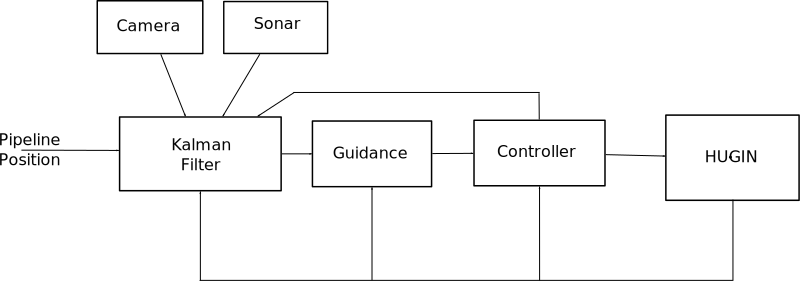
\includegraphics[width=0.9\textwidth]{pics/blockdiagram}
		\caption{Block diagram the path following controller}
		\label{fig:ch2-blockdiagram}
	\end{figure}
	As outlined in Figure \ref{fig:ch2-blockdiagram} the building blocks of the pipeline following
	control system are the cruising controller, guidance system and the filter
	which fuses the known data about the pipeline and the measured pipeline data. To recreate the 
	pipeline coordinates in three dimentions the distance to the sea bottom is measured by a sonar. The
	filter uses prior knowledge about the pipeline to-be-followd which can be inaccurate. The filter then
	uses this together with the altitude information and camera output to estimate the position of the
	pipeline. If the pipeline should be lost at any time the filter will try to predict where the pipeline
	are and serve as input to the guidance system.
	
	The system should be able to handle burried sections of the pipeline. The camera will not be able to
	sense the pipeline during the burried strech and other sensors have to be included. A bottom
	penetrating sonar might be used for this purpose, or a magnetic pipe tracker. These sensors are able
	to sense the pipeline even if burried up to 3 meters. \cite{PhD_lecture} This sensors will give the
	AUV better chances to regain track after the burried strech than if it were to relay on just dead
	recogning from the predicted pipeline information alone.

\section{Pipeline representation}
	The representation of the pipeline is important because it is used in the Kalman filter to predict
	where the pipeline is going. The pipeline is parametrized by $\varpi \in \mathbb{R}$ to get a
	continous and smooth pipeline.

	In this report the pipeline are parameterized as:
	\begin{equation}
		P_w(\varpi) = \left [ \begin{array}{c}
					\varpi \\
					k_y \varpi \\
					z(\eta)
				\end{array} \right ] \quad \varpi \in (0, \infty)
	\end{equation}
	where $k_y$ are constant and $z(\eta)$ is some function described by the sea bottom and are assumed
	known. This represents the straight line as the pipeline are assumed to be.
	
	


\section{Kalman filter}
	The Kalman filters purpose is to smooth the camera output and predict forward where the pipeline will
	be in the future to supply a better heading reference for the guidance controller.

	The position of the pipeline are given some uncertanty becuase the pipeline may have moved after it
	was layed or the navigation system of the AUV might be erronous. This gives:
	\begin{equation}
		P_w(\varpi) = \left [ \begin{array}{c}
					\varpi \\
					k_y \varpi \\
					z(\eta)
				\end{array} \right ] + \mathbf{B}\delta
	\end{equation}
	The function $\delta$ are a slowly varying disturbance which can be modeled as a \textit{1st order Markov
	Process}, and $\mathbf{B}$ is some 2x3 matrix.
	\begin{equation}
		\dot{\delta} = -\mathbf{T} \delta +  w
	\end{equation}
	where $w \in \mathbb{R}^2$, are a zero mean unity variance white noise process. This describes the
	error in the position. The matrix $\mathbf{T}$ specifies how the error evolves. Because the error are
	slowly varying the eigenvalus of $\mathbf{T}$ should be chosen large. Time differentianting
	the position estimate with regard to time gives
	\begin{equation}
		\dot{P_w}(\varpi) =  \left [ \begin{array}{c}
						\dot{\varpi} \\
						k_y \dot{\varpi} \\
						\dot{z}(\eta)
					\end{array} \right ] + \dot{\delta}
	\end{equation}
	By setting $\varpi = N(t)$, i.e the North position and completely disregarding the depth coordinate.
	gives the following
	\begin{equation}
		\dot{P_w'} = \left [ \begin{array}{c}
					n \\
					k_y n 
				\end{array} \right ] + \dot{\delta}
	\end{equation}
	Choseing the state vector and input as:
	\begin{equation}
		x = [ P_w'^T \quad \delta^T]^T \quad \Rightarrow  \quad \dot{x} = [\dot{P_w'^T} \quad
		\dot{\delta^T}]^T \quad  u = n
	\end{equation}
	This calls for the following state space representation 
	\begin{equation}
		\dot{x} = \left [ \begin{array}{cc}
					0 & -T \\
					0 & -T
				\end{array} \right] x + \left [ \begin{array}{c}
								1 \\
								k_y\\
								0 \\
								0
								\end{array} \right] u +
				\left [ \begin{array}{c}
						\mathbf{0}_{2x2} \\
						\mathbf{I}_{2x2} 
					\end{array} \right] w
	\end{equation}

	The measurement model are more complex. In order to compare the measurement from the camera with the
	state space model, the perspective equations from Section \ref{ch1-cameramodel} are needed. By using
	Equations \eqref{eq:ch1-P_c} and \eqref{eq:ch1-perspective}, we can transform the point from World
	coordinates to image coordinates. We want $y = P_i$
	\begin{equation*}
		y = P_i = \mathbf{H} P_c = \mathbf{H R}^T ( P_w - O(t))
	\end{equation*}
	$O(t)$ is the origin of the camera frame and is equal to the position vector $\eta' = [N(t),
	E(t)]^T$ of the AUV in the NED frame. By including the position vector in the input to the filter and using 
	$P_w = \mathbf{C} x$, the measurement model are conclueded.
	\begin{equation}
		\label{eq:ch2-measurement}
		y = \mathbf{H R}^T \mathbf{C} x - \mathbf{H R}^T  O(t) = \mathbf{C}'x + \mathbf{D} u
	\end{equation}
	where $\mathbf{C'}$ and $\mathbf{D}$ are apropriate matrices for selecting the right states. $\mathbf{R}$
	are the Rotation Matrix from World coordinates to Camera coordinates. This gives the following model
	for the Kalman filter
	\begin{align}
		x &= \mathbf{A} x + \mathbf{B} u + \mathbf{E} w\\
		y &= \mathbf{C}'x + \mathbf{D} u + v\\
		\mathbf{A} &= \left [ \begin{matrix}
					0 & 0 & -T_1 & 0 \\
					0 & 0 & 0 & -T_2 \\
					0 & 0 & -T_1 & 0 \\
					0 & 0 & 0 & -T_2 
					\end{matrix} \right] \quad \mathbf{B} = \left[ \begin{matrix}
										1 & 0 & 0 \\
										k_y & 0 & 0\\
										0   & 0 & 0 \\
										0 & 0 & 0
										\end{matrix} \right]\\
		\mathbf{E} &= \left [ \begin{matrix}
					0 & 0 \\
					0 & 0 \\
					1 & 0 \\
					0 & 1
					\end{matrix} \right] \quad \mathbf{C}' = \left [ \begin{matrix}
						\frac{f}{z_c} \cos{\psi} &\frac{f}{z_c} \sin{\psi} & 0 & 0 \\
						-\frac{f}{z_c} \sin{\psi}& \frac{f}{z_c} \cos{\psi} & 0 & 0 
								\end{matrix} \right] \\
		\mathbf{D} &= \left [ \begin{matrix}
					0 & -\frac{f}{z_c} \cos{\psi} & -\frac{f}{z_c} \sin{\psi} \\
					0 & \frac{f}{z_c} \sin{\psi} & -\frac{f}{z_c} \cos{\psi}
					\end{matrix} \right]
	\end{align}
	$w, v$ are a vectors of unity white noise and have covariance $E(ww^T) = \mathbf{Q}$ and $E(vv^T) =
	\mathbf{W}$. The filter should be run at the same frequency as the guidance system to provide output
	for the guidance system. The prediction will be updated whenever possible, which means when the
	pipeline are visible in the camera after the image processing are done.

	Because of the relatively high frequency of the filter the parameters in the measurement model
	regarding heading and depth, i.e. $\psi$ and $z_c$ can be assumed constant during the sample period.
	This due to the slow dynamics of the AUV, compared to filter rate. This gives a linear model which can
	be guarantead to be optimal for the current case.


\section{Controller Design}
	The model discussed in Section \ref{sec:ch1-model} is used to derive the controller equations for the
	AUV control system.

	The control system which supply the lower-level control system with forces and moments references, is 
	divided into 3 sub systems:
		\begin{itemize}
			\item Speed control
			\item Depth control
			\item Heading control
		\end{itemize}
	This is called the flightmode controller, which is used for normal pipeline tracking, descent and
	ascent. This type of controller where chosen because it will be more energy efficient than other more
	actuated controllers. The second reason is even if the AUV is almost fully actuated, i.e
	controllable in 5 DOF, the tunnel thrusters which have to be present for this degree of actuation are almost
	usless for higher velocities. This renders just control in 3 DOF, \textit{surge, pitch} and
	\textit{yaw}. This will probably give the most energy efficient pipeline following, because the
	control are based on the cheapest control modes available at the AUV.
	
	The \textit{HUGIN}-type AUV is a slender-body type AUV. This makes it possible to neglect some
	coupling effects between the states in the dynamic model. The \textit{longitudinal} states 
	(\textit{surge, heave, pitch}) can be decoupled from the \textit{lateral} states 
	(\textit{sway, roll, yaw}). This will be utilised in the next sections when deriving the control model
	and controller.

	All coefficient next are defined in accordance with \cite{SNAME}.
	\subsection{Speed Controller}
		The speed controller is derived form the \textit{surge}-subsystem, called \textit{surge}-model
		\cite{fossen}. Under the slow speed assumption, the coriolis/centripetal-matrix is assumed
		zero, $\coriolis \approx 0$  
		\begin{equation}
			(m - X_{\dot{u}})\dot{u} - X_u u - X_{|u|u}|u| u = \tau_1
		\end{equation}
		Setting $\tau_1 = -K_p \tilde{u} - K_i \int \tilde{u} dt - K_d \dot{u}$ the error in the velocity
		reference will go to zeros. The velocity reference is assumed constant and the PID controller
		guarantees that the error will go to zero.
	
	
	
	\subsection{Depth Controller}
		To derive the depth controller in the crusing control system the
		\textit{longitudinal}-subsystem is used as the control model \cite{fossen}. By assuming that the lateral
		states i.e $v, p, r, \phi$, are small, the kinematics can be derived as follows:
		\begin{equation}
			\left [ \begin{matrix}
					\dot{d} \\
					\dot{\theta}
				\end{matrix} \right] = \left [ \begin{matrix}
								\cos{\theta} & 0 \\
								0 & 1
								\end{matrix} \right] 
						\left[ \begin{matrix}
								w \\
								q
							\end{matrix} \right]
						+ \left [ \begin{matrix}
								-\sin{\theta}\\
								0
							\end{matrix} \right] u
		\end{equation}
		The dynamics of the system then becomes
		\begin{equation}
			\begin{aligned}
				\left [ \begin{array}{ccc}
					m - X_{\dot{u}} &  X_{\dot{w}} & m z_g - X_{\dot{q}} \\
					X_{\dot{w}} & m - Z_{\dot{w}} & m x_g - Z_{\dot{q}} \\
					m z_g - X_{\dot{q}} & m x_g - Z_{\dot{q}} & I_y - M_{\dot{q}} 
					\end{array} \right]
				\left [ \begin{array}{c}
					\dot{u} \\
					\dot{w} \\
					\dot{q} 
					\end{array} \right] \\
				+ \left [ \begin{array}{ccc}
					-X_u	&	-X_w 	&	-X_q \\
					-Z_u	&	-Z_w	&	-Z_q \\
					-M_u	&	-M_w	&	-M_q
					\end{array} \right]
				\left [ \begin{array}{c}
					u \\
					w \\
					q 
				\end{array} \right] + 
				\left [ \begin{array}{ccc} 
					0 & 0 & 0 \\
					0 & 0 &  -(m - X_{\dot{u}}) u \\
					0 & (Z_{\dot{w}} - X_{\dot{u}}) u & m x_g u 
					\end{array} \right]	
				\left [ \begin{array}{c}
					u \\
					w \\
					q 
				\end{array} \right] \\
				+  \left [ \begin{array}{c}
					0 \\
					0 \\
					W z_b \sin \theta \\
					\end{array} \right] = \left [ \begin{array}{c}
									\tau_1 \\
									\tau_3 \\
									\tau_5
								      \end{array} \right ]
			\end{aligned}
		\end{equation}
		Since the \textit{surge}-speed are stabilized with the controller derived in the previous
		section, the surge equation can be removed from the system under the assumption $u = u_0$.		
		Also by asuming that the \textit{heave}-velocity and $\theta$ are small the control model
		becomes:
		\begin{equation}
			\left [ \begin{matrix}
					\dot{d} \\
					\dot{\theta} \\
					\dot{q} 
				\end{matrix}
				\right ] = \left [ \begin{matrix}
							0 & -u_0 &  0 \\
							0 & 0 &   1 \\
							0 & -\frac{1}{\gamma} W &-\frac{1}{\gamma}M_{w} 
							(m - Z_{\dot{w}})-M_w Z_q
						\end{matrix} \right ] 
				\left [ \begin{matrix}
						d \\
						\theta \\
						q
					\end{matrix} \right] + \left [ \begin{matrix}
										0 \\
										0 \\
										\frac{1}{\gamma}
									\end{matrix} \right] \tau_5
		\end{equation}
		where $\gamma = m I_y - m M_{\dot{q}} - I_y Z_{\dot{w}} + Z_{\dot{w}} M_{\dot{q}}$.
		
		When closing the loop the following is proposed PID-like controller
		\begin{equation}
			\begin{aligned}
				\tau_5 &= -K_{dp} \tilde{d} + K_{dd}  \theta + K_{dd2} q \\
				\tilde{d} &= d - d_d \quad \dot{\tilde{d}} = -u_0\theta \quad
				\ddot{\tilde{d}} = -u_0q
			\end{aligned}
		\end{equation}
		A similiar controller are implemnted in \cite{NDRE-AUV}.
				

	
	\subsection{Heading Controller}
		Using the \textit{lateral}-subsystem representation from \cite{fossen}. Under the assumtions
		that $w, p, q, r, \phi,$ and $\theta$ from the longitudinal subsystem are small, the
		kinematics are reduced to:
		\begin{align}
			\dot{\phi} &= p \\
			\dot{\psi} &= r 
		\end{align}
		The low-speed assumtion is utilized, higher order velocity terms are neglected, and
		constant \textit{surge}-velocity $u = u_0$ are| assumed. This gives the following system:
		\begin{equation}
			\begin{aligned}
				\left [ \begin{array}{ccc}
					m - Y_{\dot{v}} & - m z_g - Y_{\dot{p}} & m x_g - Y_{\dot{r}} \\
					-m z_g - Y_{\dot{p}} & I_x - K_{\dot{p}} & I_{zx} - K_{\dot{r}} \\
					m x_g - Y_{\dot{r}} & I_{zg} - K_{\dot{r}} & I_z - N_{\dot{r}} 
					\end{array} \right]
				\left [ \begin{array}{c}
					\dot{v} \\
					\dot{p} \\
					\dot{r} 
					\end{array} \right] \\
				+ \left [ \begin{array}{ccc}
					-Y_v	&	-Y_p 	&	-Y_r \\
					-M_v	&	-M_p	&	-M_r \\
					-N_v	&	-N_P	&	-N_r
					\end{array} \right]
				\left [ \begin{array}{c}
					v \\
					p \\
					r 
				\end{array} \right] + 
				\left [ \begin{array}{ccc} 
					0 & 0 & (m - X_{\dot{u}})u \\
					0 & 0 &  0 \\
					(X_{\dot{u}} - Y_{\dot{v}}) u & 0 & m x_g u 
					\end{array} \right]	
				\left [ \begin{array}{c}
					v \\
					p \\
					r 
				\end{array} \right] \\
				+  \left [ \begin{array}{c}
					0 \\
					W z_b \sin \phi \\
					0 
					\end{array} \right] = \left [ \begin{array}{c}
									\tau_2 \\
									\tau_4 \\
									\tau_6
								      \end{array} \right ]
			\end{aligned}
		\end{equation}
		The \textit{roll}-state can be removed from the equations because of the assumtions of small
		$\dot{p}, p$ and because of the vessel are considered stabel in roll because of
		the offset in the bouyancy point. The \textit{sway}-velocity can assumebly be neglected, 
		the sway subsystem can be removed as well.  This can be seen from the simulations later 
		in the report. 

		The following control model are used to derive the heading controller. The model is really
		the 1st order Nomoto model, and have become famous for it simplicity yet prove to give good
		results. 
		\begin{equation}
			\left [ \begin{matrix}
					\dot{\psi} \\
					\dot{r}
				\end{matrix} \right]  =  \left [ \begin{matrix}
								0 & 1 \\
								0 & \frac{N_r - m x_g u_0}{I_z - N_{\dot{r}}}\\
								\end{matrix} \right] 
							\left [ \begin{matrix}
									\psi \\
									r
								\end{matrix} \right]
							+ \left [ \begin{matrix}
									0\\
									\frac{1}{I_z - N_{\dot{r}}}
								\end{matrix} \right] \tau_6
		\end{equation}

		The following heading controller are proposed:
		\begin{equation}
			\tau_6 = T\dot{r_d} + r_d - K_{hp} \tilde{\psi} - K_{hi} \int \tilde{\psi} dt - K_{hd}
			\dot{\tilde{\psi}}
		\end{equation}
		The terms $T \dot{r_d} + r_d$ are reference feed forward terms which will guarantee perfect
		tracking during course-changing maneuvers according to. This requiers a smooth reference
		signal and care must be taken to calculate it. \cite{fossen} 


\section{Summary of Assumtions}
	A summary of the assumtions are given here:
	\begin{enumerate}
		\item The pipeline is layed on the sea bottom, which gives the pipeline the same
		height signature as the sea bottom. The guidance problem is then reduced to a
		two-dimentional problem. No free-spanning pipelines are present.
		\item Pitch- and roll angles, are assumed small together with the corresponding pitch- and
		roll rates. In the vicinity of $\pm 10^{\circ}$ and $\pm 0.05 \mathrm{rad/s}$
		\item \textit{sway} and \textit{heave} velocities are small compared to \textit{surge}
		velocity and any cross-coupling terms may be neglected.
		\item The full state are assumed perfectly known, i.e. velocity and acceleration of the AUV.
		\item The exact position of the are known.
	\end{enumerate}
		


\section{Guidance system}
	An autonomous system is by definition a system that will have minimal interaction from humans, it is
	supposed to do things on its own. This is the guidance systems task.
	Figure \ref{fig:ch2-Guidance-block} shows a proposal of a guidance and descision system for 
	the \hugin vehicle.
	\begin{figure}[htbp]
		\centering
		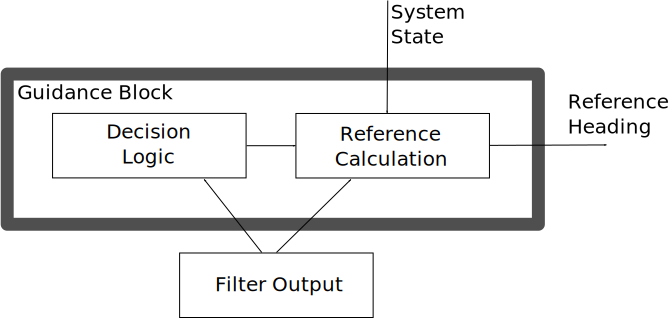
\includegraphics[width=0.8\textwidth]{pics/guidance}
		\caption{Guidance System Block}
		\label{fig:ch2-Guidance-block}
	\end{figure}

	The AUV guidance system are assumed to have three modes, \textit{searching}, \textit{tracking} and
	\textit{initialize/finalize}. The \textit{initialize/finalize}-mode are the beginning and end of a
	mission and will not be considered in this report. 
	
	The \textit{searching}-mode are when the AUV are looking for the pipeline. When the pipeline are layed
	on the sea floor, the position may be more or less inexact. Both because of sometimes the great 
	distance from the sea level and to the sea bottom, and sometimes because the pipeline have ``sagged'', 
	i.e moved away from the initial position because of movement in the sea bottom caused by sea currents
	and other environmental forces. 

	\begin{figure}[htbp]
		\centering
		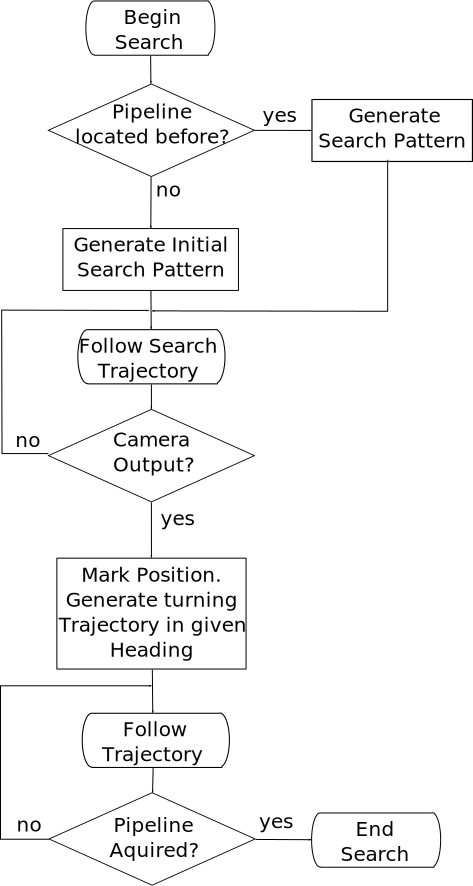
\includegraphics[width=0.5\textwidth]{pics/search_flow}
		\caption{Flow diagram of the search procedure in the \textit{searching}-mode}
		\label{fig:ch2-search-flow}
	\end{figure}
	Figure~\ref{fig:ch2-search-flow} shows the searching procedure. It shows the descisions that the
	descion block need to handle. The system distinguishes between the cases if the pipeline have been
	located before, or not. If the pipeline have not been located before, the system generates a initial
	search pattern, which should be designed to cover larger area. If on the other hand the pipeline have
	been located before, and tracking have been initialised, another pattern should be generated. The
	system then follows this search pattern until it gets output from the camera, or other possible
	sensors. Then the position are marked and a turning trajcetory are generated. When the pipeline then
	is reaqcuired the guidance system goes to the tracking mode.
	\begin{figure}[htbp]
		\centering
		\includegraphics[width=0.4\textwidth]{pics/contact_trajectory}
		\caption{A turning trajectory for one possible contract}
		\label{fig:ch2-turning-trajectory}
	\end{figure}
	
	When in the \textit{tracking}-mode the AUV tries to follow the pipeline as closly as possible, and
	keep the pipeline inside the field of view as best as possible.

	\subsection{Reference Calculation}
		A look-ahead based guidance algorithm is chosen for it's simplicity and robustness. All
		together a pipeline are made up of mostly linear segments or at least almost linear
		segment. One can then assume that the direction of the pipeline can be known exact.
		No sudden turns are assumed and pipeline junctions are assumed to be non excisitng. This gives
		the following equations, some are treated in Chapter~\ref{chap1-guidance-alg}.
		\begin{align}
			\psi_d &= \alpha_k + \psi_r \\
			\psi_r &= \tan^{-1} \left( \frac{-e}{\Delta} \right)\\
			e &= -(n(t) - p_x)\sin\alpha_k + (e(t) - p_y) \cos\alpha_k
		\end{align}
		
		In the presence of ocean current it will cause the heading to ``lean'' towards the current if
		the look-ahead distance is not chosen too far away. There will be some kind of equalibirium
		between the current and the AUV heading. This will will work well under the assumption that
		the current are constant.
		
	
	\subsection{Search Patterns}
		\label{subsec:ch2_searchpattern}
		It is obvious that some kind of search pattern must be implemented for this kind of
		application. This might be customized for every mission or it might be selected from a library
		of suiting search patterns. 
		This section will look at some search patterns which might be suiting for the pipeline search
		application.

		\begin{figure}[htbp]
			\centering
			\subfigure[Divergent Zig-Zag pattern for lost pipeline during tracking]{
				\label{fig:ch2_zig_zag}
				\includegraphics[width=0.4\textwidth]{pics/divergent_zig-zag}} \quad
			\subfigure[Outwards spiral pattern for inital pipeline search]{
				\label{fig:ch2_spiral}
				\includegraphics[width=0.4\textwidth]{pics/spiral_search}}
			\caption{Differnet search pattern}
			\label{fig:ch2_searchpattern}
		\end{figure}
		The first case is when the pipeline are not in its predetermined position or the position
		sensors gives out erronous readings, some kind of search need to be initiated to find the
		pipeline. This could be something like the depicted case in Figure~\ref{fig:ch2_spiral}.
		Spiral pattern going outwards to try to find the pipeline in the visinity of the AUV position.
		This should be aided with other sensors for example with a Side Scan Sonar which provides good
		sensor data in the horizontal directions around the AUV. 

		The other case is when the pipeline are lost during tracking. Since the general direction of
		the pipeline are assumed known, the other pattern are a divergent zig-zag pattern around the
		assumed pipeline trajectory, from the last known position.

		The search pattern can be created using polar coordinates from the current position of the
		AUV. The parameters, area in the initial search pattern or the spread angle in the divergent 
		zig-zag should be customised for each mission.

	
\section{Overall System}
	The system flow are depicted in Figure~\ref{fig:ch2-flowdiagram}. This is how the overall system behaves
	during a pipeline inspection mission. 
	\begin{figure}[htbp]
		\centering
		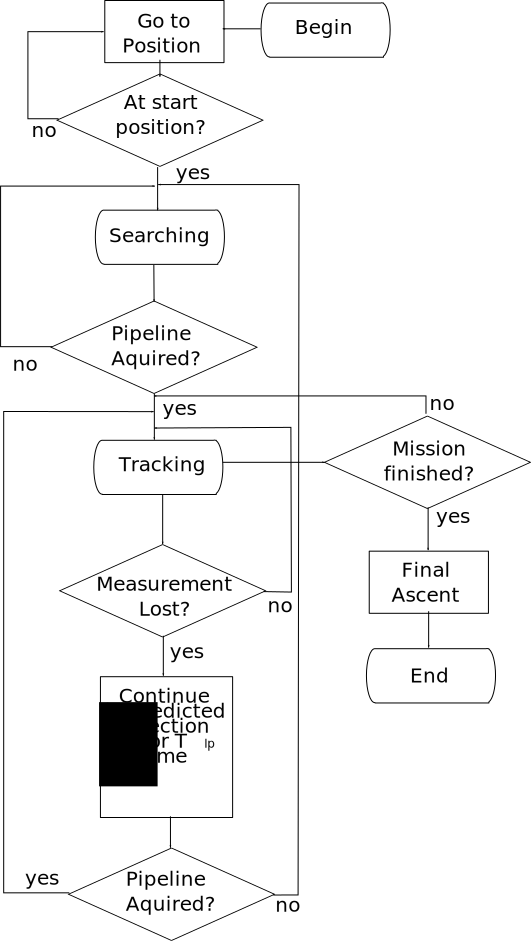
\includegraphics[width=0.5\textwidth]{pics/Operation}
		\caption{Flow diagram of pipeline inspection mission}
		\label{fig:ch2-flowdiagram}
	\end{figure}
	The system will start by moving to the point where the inspection should start. Then the searching
	procedure will be initiated if the AUV does not make contact with the pipeline imediatly. It will
	search for the pipeline until it has located it and then continue tracking until the the goal are met
	or the onboard energy storage becomes depleted. 

	There are a number of design parameters needed to be set. These parameters might be constant or
	changing between missions. They are summarised in Table~\ref{tab:ch2-design-param}
	\begin{table}[htbp]
		\centering
		\begin{tabular}{| c | p{6cm} |}
			\hline
			Design Parameter 	& 	Description \\
			\hline
			\hline
			$T_{lp}$ 		&	The Dead recogining time. Time before pipeline are
							considered lost. \\
			\hline
			$\Delta$		&	The lookahead distance, descinding the convergence of
							the heading to the path \\
			\hline
			$\alpha_k$		&	The general pipeline direction, need to be specified\\
			\hline
			$P_w$			& 	The predicted path of the pipeline in world
							coordinates or a prametrization of it \\
			\hline
			$\mathbf{T}$		&	The values of this matrix must be chosen in accordance
							with the uncertainty of the predicted pipeline path.
							Usually chosen large \\
			\hline
			$\mathbf{Q}$ \& $\mathbf{W}$ & 	The covariance matrices of how much you want to trust
							the predicted values of the pipeline and the
							uncertainty of the measured ones. \\
			\hline
		\end{tabular}
		\caption{Summary of design parameters in the system}
		\label{tab:ch2-design-param}
	\end{table}
	These parameters should be chosen in accorance with what kind of envirionmanetal forces there are in
	the area. Also the search patterns should be customised for every mission. Set how much area they need
	to cover, and vary the spreading angle of the divergent zig-zag pattern in accordance with how certain
	the direction of the pipeline are.
	


\chapter{Simulation}
	To test the performance of the guidance system, it is implemented in matlab/simulink. A number of
	scenarios are used to test how it performes in various conditions.

	The proposed system are greatly simplyfied and there are a number of situations that it will not work
	well. This situations are also threated and discussed in the next chapter. 
	

\section{Matlab}
	The mathematical model of the \textit{HUGIN 1000} AUV are implemented in simulink using the
	\textit{GNC} toolbox available from \textit{www.marinecontrol.org} with slight modifications to the
	6DOF model.

	The Camera output simulator were programmed in matlab. It inputs the position of the AUV and
	transposes it to body coordinates to calculate the field of view of the camera. The camera are based
	on the pinhole camera model with unity focus distance, and a view angle of about 45 degrees. The
	program then calculates the field of view of the camera and checks if there are any part of the
	pipeline inside the field of view. The output of the camera are three points taken out at the top, the
	middle and the bottom of the field of view.

	A sonar which determines the altitude are implemented using a look-up table with a predefined bottom
	profile.

	The descision logic is implemented as a state machine with three states, and gives out the 
	desired heading dependent on what state the system is in.

	The filter was created using a m-file and global variables for the filter parameters. The filter
	parameters are as follows:
	\begin{equation}
		P_0 = \left [ \begin{matrix}
				10 & 0 & 0 & 0 \\
				0 & 10 & 0 & 0 \\
				0 & 0 & 0.1 & 0 \\
				0 & 0 & 0 & 0.1
				\end{matrix} \right] \quad
		W = 0.1 \mathbf{I}_{2x2} \quad Q = 10 \mathbf{I}_{2x2} 
	\end{equation}

	The final simulink diagram are shown in figure \ref{fig:ch3_simulink}.
	\begin{figure}[htbp]
		\centering
		\includegraphics[width=\textwidth]{pics/simulink}
		\caption{The Simulink Diagram of the implemented Guidance System}
		\label{fig:ch3_simulink}
	\end{figure}

	

\section{Simulation Scenarios}
	To test the performance of the guidance system some scenarios are proposed.
	\begin{description}
		\item[\textbf{1$^{\mathrm{st}}$ Scenario}.] The pipeline are at the exact location acording 
		to predefined data. Environmental disturbances such as currents are turned off. The pipelien are
		continiously visible for the camera the whole inspection distance. Reference simulation.
		\item[\textbf{2$^{\mathrm{nd}}$ Scenario}.] Exact as over but with environmental forces turned on.
		\item[\textbf{3$^{\mathrm{rd}}$ Scenario}.] The pipeline are at the exact location where 
		it initially was layed. A section is burried, and not visible for the camera. Environmental
		forces are turned on.
		\item[\textbf{4$^{\mathrm{th}}$ Scenario}.] The \'a priori information about the pipeline 
		are offset about 20 meteres to test the ability of the guidance system to search for the pipeline.
	\end{description}


\section{Results}
	Some of the results for the simulations scenarios are given here. But first a test of the low-speed
	assumptions made for the controller design for the AUV. 

	\subsection{Test of the low-speed assumtion}
		In figures \ref{fig:ch3_coriolis_forces} and \ref{fig:ch3_damping_forces} the forces and
		moments created by the Coriolis/centripetal and damping matrices are recorded. In Figure
		\ref{fig:ch3_coriolis_forces} the sway degree of freedom are dominant, and peaking about
		-400N during the turning maneuvers of the AUV. The forces and moments created by the coriolis
		terms are partially counteracted by the damping terms, that also have greated magnitude than
		the coriolis terms.
		\begin{figure}[htbp]
			\centering
			\includegraphics[width=0.7\textwidth]{pics/coriolis_forces}
			\caption{Plot of the Coriolis Forces Associated with the AUV Model}
			\label{fig:ch3_coriolis_forces}
		\end{figure}		
		\begin{figure}[htbp]
			\centering
			\includegraphics[width=0.7\textwidth]{pics/damping_forces}
			\caption{The Dampering Forces Associated with the AUV when Maneuvering}
			\label{fig:ch3_damping_forces}
		\end{figure}
		This suggests that the coriolis/centripetal forces can be neglected and compensated for as
		model errors in the controller using integral terms.  

	\subsection{1$^{\mathrm{st}}$ Scenario}
		This is mostly a reference test to see how the guidance system performs on the ideal case.
		This can show how sensitive the guidance system are with regard to current disturbances.
		\begin{figure}[htbp]
			\centering
			\includegraphics[width=0.7\textwidth]{pics/1st_NE_path}
			\caption{North East path of AUV without Current}
			\label{fig:ch3_1st_NE_path}
		\end{figure}
		\begin{figure}[htbp]
			\centering
			\includegraphics[width=0.75\textwidth]{pics/1st_uDpsi}
			\caption{Surge-, Depth- and Heading- Reference vs. Actual Values}
			\label{fig:ch3_1st_uDpsi}
		\end{figure}
		The result of this test is purly for reference but it might be an idea to notice some things
		about the simulations. 
		
		It can be seen from both Fiugre \ref{fig:ch3_1st_NE_path} and the
		third plot on Figure \ref{fig:ch3_1st_uDpsi} that the heading reference, $\psi_d$ have some
		oscilatory nature. This is because of the relatively low look-ahead distance defined in the
		guidance algorithm. This can be analogus to when driving a car and you fix your gaze on
		the road not very far ahead of the car, and you will get more uneasy driving and not so smooth motion. 

		The depth reference are given by the bottom which are constructed using a look-up table
		created by a sinuosidal plane. The reference are followed pretty well. The delay on the
		action by the controller are created because the \textit{heave} direction are not directley
		controlled, but are relayed through the \textit{pitch} degree of freedom.

	
	\subsection{2$^{\mathrm{nd}}$ Scenario}
	
	
	
	\subsection{3$^{\mathrm{rd}}$ Scenario}
	
	
	
	\subsection{4$^{\mathrm{th}}$ Scenario}


\chapter{Discussion}
	This chapter will summarize and discuss the results in the previous chapter.

\section{Guidance System}
	The guidacen system are greately simplifyed. In this section these simplifications will be adressed
	and other possible errors and shorcomings will be treated. 

	This Guidance system are designed for long, straight pipeline streches. It will not be able to handle
	sudden turns in the pipeline direction, without spcifying this in the guidance system. This can be
	included as waypoints where the pipeline are changing, and be included as a condition; \textit{when the AUV
	reaches certain position the direction of the pipeline changes}. This requiers very exact knowledge
	about the pipeline and are rearly the case. TThis is why there should be a more autonomous way of
	doing this. This motivates the use of more sensros than just a camera to follow the pipeline. The
	camera have a very limited field of view, usually restricted to less than 3 meters. A Side Scan Sonar
	comined wiht a Forward Looking Sonar, which provides sensor data of the pipeline in front of the AUV
	will give the guidance system some data to descide and predict what it will do if there is a sharp
	turn in the pipeline. 

	Sharp turns are rare, and are a product of T-junctions and other couplings of pipelines. These
	junctions are usually well documented, and given good and exact locations. But if the navigation
	sensors of the AUV have large uncertanties, and from the AUV it might look as they are in the wrong
	place. This suggests that information about the pipeline should be treated with care. Because the
	errors in an AUV navigation system might be substantial and provide that \'a priori information about
	the pipeline will be unusable. 

	The navigation system of \textit{HUGIN 1000} are a Velocity Aided Inertial Navigation System. This
	utilises a Doppler Velocity Log to measure the velocity relatively to the sea bottom and input this to
	the INS system. The INS systems usually installedn on the \textit{HUGIN} are in the 1 nmi/h class, i.e
	the INS system drifts less than 1 nmi/h. This results in a drift in the navigation system equal to
	0.11 \% of the traveled distance along the track, and about 0.03 \% error in the across distance of a
	stright line track. \cite{INS_Hugin}. This can be enough to throw the guidance system off course,
	because the field of view of the camera are relatively small.

	***********************************************

	There are ways of improving the INS drift, one is to use GPS update fixes, but this requiers to
	surface the AUV once in a while. This is of course not a good idea when the AUV are at great depths.
	There are posibilities to use sea bottom anchored position bouys, which exact position are known and
	the AUV might use these bouys by pinging them and getting a updated position estimate. This is a good
	idea if the pipeline infrastructure admints this. Say that this position bouys are placed at the same
	time as the pipeline are layed, but this is a costly affair. 

	Too use a Ultra Short Base Line (USBL) are another posibility. A USBL transducer are mounted on a
	ship, which has a GPS location fix. The AUV then pings the USBL transducer regularily and the position
	are determined exactly. This requiers a ship stationed in the area where the AUV are carrying out the
	mision. The autonomicity of the AUV are the reduced, and the vehicle are not capable of operating on
	its own. 

	**********************************************

	The problem regarding when $\psi \rightarrow 2\pi$ problem, there are a number of solutions for this.
	The first is to limit the sensor output, which are the case in the real world, since a compass
	measuring \textit{yaw} only are defined for $(0, 2 \pi)$. The controller can handle this by including
	a chech wheter if its heading are larger than $\pi$, the given command will be to the right, and
	opposite if the measured heading are smaller than $\pi$.

	\subsection{Increasing the inspection speed}
		What happens when the inspection speed are increased beyond 1 m/s? Say if the surge velocity
		were to be increased to 2 m/s. 




\section{Roll Stabilization}
	The mission of the AUV are to provide good data for later use, i.e good pictures to be analyzed later.
	The camera on the AUV are mounted downwards and the field of view are affected by roll and pitch.
	Pitch are a contorl angle, but the Roll motion have no direct control measures. The roll angle need to
	be as close to 0 as possible to provide best pictures of the current sea bottom. Imagine if the AUV
	were to move upside-down above the sea bottom. The plots in Figure~\ref{fig:ch4_rollyawmoment}
	are taken from the $4^{\mathrm{th}}$ Scenario described in Chapter~\ref{ch3}, to look at \textit{HUGIN
	1000}'s stability in roll.
	
	\begin{figure}[htbp]
		\centering
		\subfigure[Roll Angle]{
			\label{fig:ch4_rollangle}
			\includegraphics[width=0.7\textwidth]{pics/ch4_rollangle}}
		\subfigure[Yaw Moment]{
			\label{fig:ch4_yawmoment}
			\includegraphics[width=0.7\textwidth]{pics/ch4_yawmoment}}
		\caption{Plots describing the close relation of yaw moment and roll angle}
		\label{fig:ch4_rollyawmoment}
	\end{figure}
	Figure~\ref{fig:ch4_rollyawmoment} shows the relation between commanded yaw moment and the roll angle.
	Clearly there are coupling effects which causes the roll angle to change a few degrees. The roll angle
	magnitude are about $2^\circ$ when the \textit{surge}-velocity are 2 m/s. But the roll angle are not
	of greate concern when carrying out this kind of inspection missions, as these simulations show.

	
	The main propeller gives a moment in roll. This moment are disregarded in the simulations, but might
	become important. The main propeller are described by the followin relations
	\begin{equation}
		\begin{aligned}
			\tau_1 &= T_{nn} n^2 + T_{un} n u \\
			\tau_4 &= Q_{nn} n^2 + Q_{un} n u
		\end{aligned}
	\end{equation}
	where $n$ are the angular speed of the main propeller in Revolutions per minute, and $u$ are again the
	surge velocity. 
	
	This moment are actually countered by weightin the AUV down on one side so that when the it reaches cruice
	velocity the AUV have zero roll angle. \cite{Bjorn_gjelstad_talk}

	This is of course due to some of the design features of \textit{HUGIN} AUV. It is designed to be
	asymptotically stable in roll, due to the centre of bouyancy (CB) are located not exactly in the centre of
	gravity (CG). The AUV would not need roll stabilisation becuase it shows to be very stable in roll.
	Another case is that if roll stabilisation were to be implemented it would be done by using the
	rudders, and this would cause an increase in power consumption that would not be advisable. 


\section{Energy Consumption}
	The energy consumption of an AUV are of extreme importance. When a customer are buying this type of
	vessel one of the criteria are operation time. For an AUV which are untethered and have limited power 
	supply the operation time might vary greatly due to installed sensors and operating conditions.

	The standard sensor suite on the \hugin AUV are a Side Scan Sonar, Doppler Velocity Log, Depth meter,
	Multibeam Echosounder, and the INS navigation system. The operation time would be around 10-20 houres,
	dependent on velocity and sensor use. The main objective of the guidance system after the inpsection
	part is to maximise the operating time. This can be done in numerous ways, and should be a part of the
	design procedure when designing the guidance system for the real thing.

	The actuator set-up of \hugin  are with 4 rudders, one main propeller and 4 thurusters. This renders
	the AUV controllable in 5 DOFs. The thrusters demand more power than the main propeller
	and rudders, and have been completely disregarded throughout this report. The most energy efficient
	way of moving is using the main propeller and the rudders to navigate the AUV.

	The most energy efficient way of guiding an AUV is to use its main propeller and rudders. But there
	might be different ways of optimising the power consumption with regard to how the AUV are searching
	for and tracking the pipeline. The forces produced by for instance the vertical rudders, the moment
	produced by this rudders are proportional to the surge velocity squared.
		\begin{equation}
			\tau_6 = Y_{u\psi} \delta u^2
		\end{equation}
	where $\delta$ are the angle of the rudder, and $Y_{u \psi}$ are some constant describing the rudder
	areal. This means that the effect of the rudders are greatly dependent on the forward speed. This is
	not taken into account in the designed controller and have to be compensated in a more advanced
	controller, or it can be taken care of in the control allocation problem not considered in this
	report.  
	
	


\section{Optimal Search Pattern}






\chapterstyle{section}
\chapter{Conclusions}






\section{Further Work}
	Topics for further work and testing:
	\begin{itemize}
		\item Obstacle aviodence
		\item Roll Stabilization
		\item Optimal guidance and path planning
		\item Learing algoritmes, Generic algoritms for obstacle  aviodance and advanced path
		planning.
	\end{itemize}




\chapterstyle{default}

\bibliography{exbib}

%%%%%
% Many appendices
%%%%
\appendices
\appendixpage
\chapter{Moderately Important Stuff}
\section{About Appendices}
If you have many appendices, do it like this: A page signifying the start of the appendices saying ``Appendices'', then the appendices numbered A, B, C, \ldots

If you only have one appendix, do not have a page saying ``Appendices''. Have just one unnumbered chapter with title ``Appendix'', or ``Appendix: Name of Appendix''. 

\chapter{More Moderately Important Stuff}%Use for many appendices


%\backmatter
%%%%%
% Only one appendix
%%%%
\chapter{Appendix: Matlab Scripts}
\section{The Descision block}
\lstset{language=Matlab, basicstyle=\tiny}
 
\begin{lstlisting} 
function y = descicion(u)
    
    global WP pipeline_dir trajectory_generated
    
    %input: Output, eta, Pipeline trajectory,
    eta = u(1:6);
    nu = u(7:12);
    p = u(13:21);
    heading = u(22);
    output = u(23);
    t = u(24); %current time
    
    lookahead = 5; %5
    lookahead_s = 12; %6
    
    persistent mode current current_s detected_pos time_since_contact last_known_pos
    % mode = 2 goto; mode=1 serach; mode = 0 track
    
    if isempty(mode) || isempty(current) || isempty(detected_pos) || isempty(current_s)
        mode = 2; %start in goto mode
        current = 2;
        current_s = 2;
        WP = [eta(1:2), WP];
        detected_pos = [0; 0];
        time_since_contact = 0;
        trajectory_generated=0;
        last_known_pos = [0 ; 0];
    end
    
    
    
    
    switch mode
        
        case 2 %goto mode
            r2 = sqrt((WP(1,current)-eta(1))^2 + (WP(2,current)-eta(2))^2);
            y = atan2(WP(2, current)- eta(2), WP(1, current) - eta(1));
               if r2 <= 5
                  current = current +1
                  
                  if output == 1
                      mode = 0
                      detected_pos = p(4:5)
                      return;
                  else
                      mode = 1
                      return;
                  end
               end

            
        case 1 %search mode Generate trajectory
            if output == 1 % && trajectory_generated ~= 1
                detected_pos = p(1:2)
                y = atan2(detected_pos(2) - eta(2), detected_pos(1) - eta(1))
                mode = 0
                trajectory_generated = 1
                return
            else
               if trajectory_generated == 2
                    [WP, current_s] = generate_WP(last_known_pos, pipeline_dir);
               elseif trajectory_generated == 0
                   [WP, current_s] = generate_initial_search(WP(1:2, 2));
               end
               

               r2_t = sqrt((WP(1,current_s)-eta(1))^2 + (WP(2,current_s)-eta(2))^2);
               
               if r2_t <= 6
                  current_s = current_s + 1
               end
               xi_wp = atan2(WP(2, current_s)-WP(2, current_s-1), WP(1, current_s)
 				 		- WP(1, current_s-1));
               
               if xi_wp < 0 %fix for not turning all the way around
                   xi_wp = xi_wp + 2*pi;
               end
               
               e = -(eta(1) - WP(1, current_s-1))*sin(xi_wp) + (eta(2) 
						- WP(2, current_s-1))*cos(xi_wp);
               y = xi_wp + atan2(-e, lookahead_s); 
               
               if output == 1 && (trajectory_generated == 1 || trajectory_generated == 3)
                   mode = 0;
                   return;
               elseif output == 1
                   mode = 0
                   detected_pos = p(4:5)
                   trajectory_generated = 1
                   return;
               end
               
            end

        case 0 %track mode
            xp = heading;
            if output == 0
                 %lost measurement
                 if time_since_contact == 0
                     time_since_contact = t
                     last_known_pos = p(4:5);
                 end
            end
            
            if abs(xp-eta(6)) > pi/2
                xp = -xp;
            end

            e = -(eta(1) - p(1))*sin(eta(6)) + (eta(2) - p(2))*cos(eta(6));

            xr = atan2(-e, lookahead);

            psi_d = xp + xr;
            y = psi_d;
            
            if t - time_since_contact == 25 %60 scn3 %25 scn 1 og 2 og 4
                mode = 1 %search mode
                time_since_contact = 0;
                trajectory_generated = 2;
                return;
            end 

    end
    last_psi_d = y;
end


function [waypoint, current] = generate_WP(eta_t, pipeline_dir)
    
    global trajectory_generated
    
    %position from origo of NED
    r1 = 80;
    r2 = 100;
    r3 = 200;
     
    %Search boundaries
    theta_min = pipeline_dir - pi/20;
    theta_max = pipeline_dir + pi/20;
    
    waypoint = [eta_t(1), eta_t(1)+r1*cos(theta_max), eta_t(1)+r2*cos(theta_min),
 				eta_t(1)+r3*cos(theta_max);
                eta_t(2), eta_t(2)+r1*sin(theta_max), eta_t(2)+r2*sin(theta_min), 
				eta_t(2)+r3*sin(theta_max)]
    
    trajectory_generated = 1;
    current = 2;
    
end


function [waypoint, current] = generate_initial_search(eta_0)
    %generate spiral pattern around initial condition.
    global trajectory_generated
    theta = 0:0.1:8*pi; %4 omdreininger
    b = 30;
    r = theta + b*theta; %spiral i polarkoordinater
    [x, y] = pol2cart(theta, r);
    waypoint = [eta_0(1); eta_0(2)];
    for i = 1:15:size(x, 2)
         waypoint = [waypoint, [eta_0(1)+x(i); eta_0(2)+y(i)]]
    end
    trajectory_generated = 1;
    current = 2;
    
end

function [waypoint, current] = generate_turn_trajectory(detected_pos, eta_t, pipeline_dir)
    %takes in detected point, pipeline direction and wp vector
    %outputs new wp vector with new wps
    
    global trajectory_generated
    psi = eta_t(6);
    
    r1 = 20;
    r2 = 50;
    r3 = 60;
    r4 = 60;
    if psi > pi/2
        theta1 = psi + pi/6;
        theta2 = psi + pi/3;
        theta3 = psi + 2*pi/5;
        theta4 = psi + 2*pi/3;
    else
        theta1 = psi - pi/6;
        theta2 = psi - pi/3;
        theta3 = psi - 2*pi/5;
        theta4 = psi - 2*pi/3;
    end
    
     if (psi > pipeline_dir + pi/8) || psi < (pipeline_dir - pi/8)
        waypoint = [eta_t(1), eta_t(1)+r1*cos(theta1), eta_t(1)+r2*cos(theta2), 
		eta_t(1)+r3*cos(theta3), detected_pos(1), detected_pos(1)+r2*cos(pipeline_dir);
                    eta_t(2), eta_t(2)+r1*sin(theta1), eta_t(2)+r2*sin(theta2), 
		eta_t(2)+r3*sin(theta3), detected_pos(2), detected_pos(2)+r2*sin(pipeline_dir)]
     else
         waypoint = [eta_t(1), detected_pos(1);
                     eta_t(2), detected_pos(2)];
     end
    
    trajectory_generated = 3
    current = 2;
    
    
end
\end{lstlisting}

\section{Camera Simulator}

\begin{lstlisting}
function [x] = camsim3(u)

%% Initialization
global pipeline focus

t = u(32);
noise = u(33);
variance = u(34);

DimX = 400;
DimY = 400;



persistent output isOutput



if mod(t, 1) == 0 %Every 1 second there is a new sample
    eta = u(1:6);
    bottom = u(13);
%% Rotation matrix
    Rot = [u(14:16) u(17:19) u(20:22)];

    Trans = [u(23:25) u(26:28) u(29:31)];


    %% Check if pipeline is inside FOV

    z = bottom - eta(3); %altitude

    fov = z*tand(45/2);

    eta_b = Rot(1:2, 1:2)'*eta(1:2);


        x_max = eta_b(1) + fov;
        x_min = eta_b(1) - fov;
        y_max = eta_b(2) + fov;
        y_min = eta_b(2) - fov;


    pipeline_b = zeros(size(pipeline,1), 3);


    pipeline_inside = [];
    for i = 1:size(pipeline,1)

        
        if z <= 6
            pipeline_b(i,:)= (Rot'*pipeline(i,:)')';
            if (pipeline_b(i,1) <= x_max) && (pipeline_b(i,1) >= x_min) %inside x direction
                if (pipeline_b(i,2) <= y_max) && (pipeline_b(i, 2) >= y_min) %inside y direction
                    pipeline_inside = [pipeline_inside; pipeline_b(i,:)]; %#ok<AGROW>

                    %         disp('ingen punkter')
                end
            end
        else
%             disp('too dark');
        end
    end

    if isempty(pipeline_inside)
    %     disp('No points inside');
        P = zeros(6,1);
        isOutput = 0;
    else
        % convert pipeline_inside into screen cooridnates
        
        %perspektivligningene
        perspektiv = diag([(1/z)*focus (1/z)*focus]);
        
        temp = size(pipeline_inside,1);

        temparr = [];
        for i = 1:size(pipeline_inside)
            temparr = [temparr; (perspektiv*(pipeline_inside(i, 1:2)' - eta_b(1:2)))'];
        end
        [r, c, v] = find(0.05 > temparr & temparr > -0.05);
        if isempty(r)
            r = ceil(temp/2);
        end
        
        B = sortrows(temparr, 1);
        
        P = [B(1,1:2)';
             temparr(r(1),1:2)';
             B(size(B,1),1:2)'];
         isOutput = 1;
    end

    if noise == 1
    
        noise = variance.*randn(6,1);
    
        output = P + noise;
    else
        output = P;
    end
    
    x = [output; isOutput];
else
    if isempty(output)
        output = zeros(6,1);
        x = [output; isOutput];
    else
        if isempty(output)
            output = zeros(6,1);
        end
        x = [output; isOutput]; 
    end
end
\end{lstlisting}


\section{Kalman Filter}

\begin{lstlisting}
function y = kalmanfilter3(u)

global n e W Q P0 x0 focus

persistent P_apr x_apr temp

if isempty(P_apr) || isempty(x_apr) || isempty(temp)
    P_apr = P0;
    x_apr = x0;
    temp = [0; 0];
end

p = u(1:6);

eta = u(7:12);
nu = u(14:19);
z_c = u(13);

output = u(20);
t = u(21);
z_b = z_c + eta(3);

psi = eta(6);

R = [cos(psi) -sin(psi) 0;
     sin(psi) cos(psi) 0;
     0          0       1];


u = [(R(1,1:2)*nu(1:2)); R(1:2, 1:2)'*eta(1:2)];

% model equations
t1 = 1/2000;
t2 = 1/2000;
A = [0 0 -t1 0;
     0 0 0 -t2;
     0 0 -t1 0;
     0 0 0 -t2];
B = [n, 0, 0;
     e, 0, 0;
     0, 0, 0;
     0, 0, 0];
f = focus;

C = [(f/z_c)*cos(psi), (f/z_c)*sin(psi), 0, 0;
     -f/z_c*sin(psi), f/z_c*cos(psi), 0, 0];

D = [0, -f/z_c*cos(psi), -f/z_c*sin(psi);
     0, f/z_c*sin(psi), -f/z_c*cos(psi)];
     
E = [0, 0;
     0, 0;
    eye(2)];

[Ad, Bd] = c2d(A, B, 0.1);
[Ad, Ed] = c2d(A, E, 0.1);
x = [];

    x_apr = [n*eta(1);
             e*eta(1);
             x_apr(3);
             x_apr(4)];

    x = [x_apr; x_apr; x_apr];
            
    K = P_apr*C'*inv((C*P_apr*C' + W));

    x_aprm = [];
    
    for i = 1:4:12
        %predict
        x_apr = Ad*x(i:i+3) + Bd*u;
        x_aprm = [x_aprm; x_apr];
    end

    
switch output
    case 1
        for i = 1:2:6
            x_post = x_apr + K*([p(i); p((i+1))] - C*x_apr - D*u);
            x = [x; x_post(1:4)];
        end
    case 0
        %set x = x_aprm
        x = x_aprm;
end
    P_post = (eye(4) - K*C)*P_apr*(eye(4) - K*C)' + K*W*K';

   
P_apr = Ad*P_post*Ad' + Ed*Q*Ed';

if temp ~= zeros(2,1)
    pipeline_heading = atan2(abs(x(2)-temp(2)), abs(x(1)-temp(1))); %use prior estimate
  
else
    pipeline_heading = 0;
end

if mod(t,20) == 0
    temp = x(9:10);
end


%% output
y = [x_apr(1:2); z_b; x(1:2); z_b;x(5:6); z_b; x(9:10); z_b; pipeline_heading; diag(P_apr)];


\end{lstlisting}%Use if you only have on appendix

\end{document}
